\documentclass[11pt,a4paper]{article}

\usepackage[T1]{fontenc}
\usepackage[utf8]{inputenc}
\usepackage[a4paper,margin=1in]{geometry}
\usepackage{lmodern}
\usepackage{microtype}
\usepackage{setspace}
\usepackage{parskip}
\usepackage{xcolor}
\usepackage{graphicx}
\usepackage{booktabs}
\usepackage{array}
\usepackage{longtable}
\usepackage{amsmath}
\usepackage{amssymb}
\usepackage{enumitem}
\usepackage{fancyhdr}
\usepackage{hyperref}
\usepackage{caption}
\usepackage{subcaption}
\usepackage{titlesec}
\usepackage{tcolorbox}
\usepackage{float}

\hypersetup{
    colorlinks=true,
    linkcolor=blue!60!black,
    urlcolor=blue!60!black,
    citecolor=blue!60!black,
    pdftitle={NLU Assignment Report: Word Embeddings and Character-level Name Generation},
    pdfauthor={B23CS1022}
}

\definecolor{accent}{RGB}{15,76,117}
\definecolor{soft}{RGB}{236,244,250}
\definecolor{textgray}{RGB}{65,65,65}

\titleformat{\section}{\Large\bfseries\color{accent}}{\thesection}{0.6em}{}
\titleformat{\subsection}{\large\bfseries\color{accent}}{\thesubsection}{0.6em}{}
\titleformat{\subsubsection}{\normalsize\bfseries\color{accent}}{\thesubsubsection}{0.6em}{}

\pagestyle{fancy}
\fancyhf{}
\lhead{NLU Assignment Report}
\rhead{B23CS1022}
\cfoot{\thepage}

\setstretch{1.15}

\begin{document}

\begin{titlepage}
    \centering
    
\includegraphics[width=0.20\textwidth]{report_assets/iitj_logo.png}\\[0.6cm]
    {\Huge \bfseries Natural Language Understanding PA-2 Report \par}
    \vspace{0.5cm}
    {\LARGE \color{accent} Word Representation Learning and Character-level Sequence Modeling\par}
    \vspace{1.5cm}

    \begin{tcolorbox}[colback=soft,colframe=accent,width=0.9\textwidth]
        \centering
        % \textbf{Topic:} Word Representation Learning and Character-level Sequence Modeling\\[4pt]
        \textbf{Name:} \texttt{Japneet Singh}\\[4pt]
        \textbf{Roll No:} B23CS1022\\[4pt]
        \textbf{Problem 1:} Learning Word Embeddings from IIT Jodhpur Data\\[2pt]
        \textbf{Problem 2:} Character-level Name Generation using RNN Variants\\[4pt]
    \end{tcolorbox}
    

    \vfill

    % {\large \textbf{Submitted On:} \today\par}
\end{titlepage}

\tableofcontents
\newpage

% \section{Executive Summary}
% This report combines two assignment problems implemented in \texttt{prob1.ipynb} and \texttt{prob2.ipynb}.

% \begin{itemize}[leftmargin=1.5em]
%     \item \textbf{Problem 1:} A domain-specific IIT Jodhpur corpus was built from webpages and PDF documents, preprocessed, and used to train both CBOW and Skip-gram (with negative sampling) Word2Vec models.
%     \item \textbf{Problem 2:} A character-level name generation pipeline was implemented using three recurrent variants: Vanilla RNN, BLSTM, and RNN with additive attention.
%     \item \textbf{Major finding:} In Problem 1, both models learned meaningful institutional semantics but with noise in rare contexts; in Problem 2, BLSTM achieved strongest novelty but suffered severe repetition artifacts, while attention produced the most human-like names among generated samples.
% \end{itemize}

\section{Problem 1: Learning Word Embeddings from IIT Jodhpur Data}

\subsection{Objective}
To train Word2Vec embeddings on IIT Jodhpur textual data and analyze semantic structure using nearest neighbors, analogies, and 2D embedding visualizations.

\subsection{Task 1: Dataset Preparation}

\subsubsection{Data Sources}
The corpus was built by combining:
\begin{itemize}[leftmargin=1.5em]
    \item IITJ official academic and departmental webpages
    \item Research and faculty-related webpages
    \item Academic regulations and institute PDF documents
    \item Institute Newsletters
    \item Institute Annual Reports
\end{itemize}


\subsubsection{Preprocessing Pipeline}
The preprocessing implemented in code includes:
\begin{enumerate}[leftmargin=1.5em]
    \item Boilerplate and URL cleaning with regular expressions
    \item Lowercasing and normalization of key terms:
    \begin{itemize}[leftmargin=1.5em]
        \item \texttt{b.tech} $\rightarrow$ \texttt{btech}
        \item \texttt{m.tech} $\rightarrow$ \texttt{mtech}
        \item \texttt{ph.d} $\rightarrow$ \texttt{phd}
        \item \texttt{u.g.} $\rightarrow$ \texttt{ug}, \texttt{p.g.} $\rightarrow$ \texttt{pg}
    \end{itemize}
    \item Tokenization using NLTK tokenizer
    \item Lemmatization using WordNet lemmatizer
    \item Stopword filtering (NLTK + custom domain/menu stopwords)
    \item Removal of non-English/non-alphabetic artifacts and very short/very long tokens
\end{enumerate}

\subsubsection{Dataset Statistics}
The final cleaned corpus statistics :

\begin{table}[H]
\centering
\caption{Problem 1 Corpus Statistics}
\begin{tabular}{l c}
\toprule
\textbf{Statistic} & \textbf{Value} \\
\midrule
Total Documents (Webpages + PDFs) & 71 \\
Total Tokens & 640,046 \\
Vocabulary Size & 34,446 \\
% Word2Vec Vocabulary Size (after min-count and token filtering) & 10,069 \\
\bottomrule
\end{tabular}
\end{table}

\begin{table}[H]
\centering
\caption{Top-10 Most Frequent Tokens}
\begin{tabular}{l c}
\toprule
\textbf{Token} & \textbf{Count} \\
\midrule
student & 7168 \\
jodhpur & 5505 \\
research & 4695 \\
technology & 4603 \\
institute & 4470 \\
iit & 4357 \\
engineering & 4296 \\
department & 4145 \\
system & 3903 \\
science & 3604 \\
\bottomrule
\end{tabular}
\end{table}

\begin{figure}[H]
    \centering
    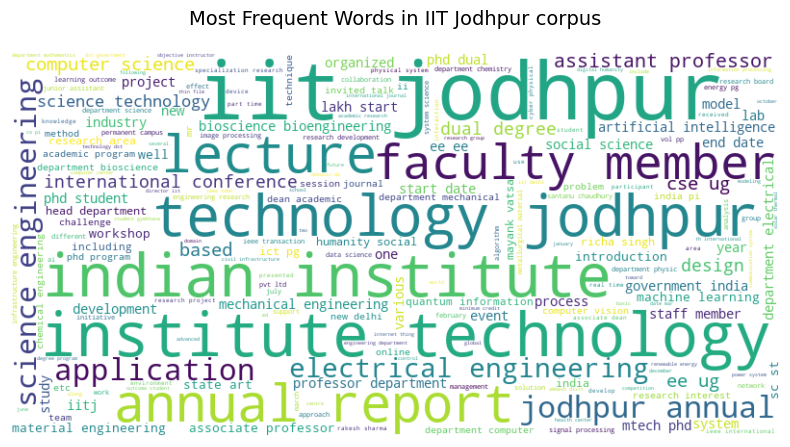
\includegraphics[width=0.96\textwidth]{report_assets/prob1_cell3_img1.png}
    \caption{Word cloud of most frequent words in the IIT Jodhpur corpus}
\end{figure}

\subsection{Task 2: Model Training (CBOW and Skip-gram with Negative Sampling)}

\subsubsection{Training Setup}
Both models were implemented from scratch in NumPy using the SGNS formulation (Skip-gram with Negative Sampling). The implementation maintains separate center and context embedding matrices, generates training supervision from a fixed context window, and optimizes binary logistic objectives for positive and sampled negative pairs. Negative tokens are drawn from a smoothed unigram distribution $p(w)^{0.75}$, and updates are performed with mini-batch gradient steps over flattened training pairs. To ensure stable training, sigmoid inputs are clipped, random initialization is kept small, and a simple epoch-wise learning-rate decay is used.

\begin{table}[H]
\centering
\caption{Word2Vec Training Configuration}
\begin{tabular}{l c}
\toprule
\textbf{Hyperparameter} & \textbf{Value} \\
\midrule
Embedding Dimension & 300 \\
Context Window Size & 5 \\
Negative Samples ($k$) & 5 \\
Batch Size & 128 \\
Epochs & 10 \\
Initial Learning Rate & 0.025  \\
Random Seed & 42 \\
\bottomrule
\end{tabular}
\end{table}


\subsubsection{Hyperparameter Experiments }

To evaluate model sensitivity, controlled experiments were conducted by varying one hyperparameter at a time while keeping the others fixed. Specifically, three ablations were run: (A) embedding dimension, (B) context window size, and (C) number of negative samples. For each setting, both CBOW and Skip-gram were retrained on the same cleaned IITJ corpus, and performance was summarized using final training loss paired with qualitative assessment of semantic quality (e.g., analogy solving capability, coherence of neighborhoods, and neighbor relevance).

\begin{table}[H]
\centering
\caption{Experiment A: Varying Embedding Dimension ($w=5, k=5$ fixed)}
\begin{tabular}{c c c c}
\toprule
\textbf{Embedding Dim} & \textbf{CBOW Loss} & \textbf{SG Loss} & \textbf{Performance} \\
\midrule
50  & 1.59 & 1.85 & Limited analogy solving capability \\
100 & 1.49 & 1.72 & Moderate improvement in semantic relationships \\
300 & 1.36 & 1.58 & Strong analogy solving, improved clustering \textsuperscript{*} \\
\bottomrule
\end{tabular}
\end{table}

\begin{table}[H]
\centering
\caption{Experiment B: Varying Context Window Size ($d=300, k=5$ fixed)}
\begin{tabular}{c c c c}
\toprule
\textbf{Window Size} & \textbf{CBOW Loss} & \textbf{SG Loss} & \textbf{Performance} \\
\midrule
3 & 1.41 & 1.63 & Limited context capture, sparse relationships \\
5 & 1.36 & 1.58 & Best coherence, balanced semantic capture \textsuperscript{*} \\
8 & 1.39 & 1.62 & Reduced coherence, noisy dependencies \\
\bottomrule
\end{tabular}
\end{table}

\begin{table}[H]
\centering
\caption{Experiment C: Varying Negative Samples ($d=300, w=5$ fixed)}
\begin{tabular}{c c c c}
\toprule
\textbf{Negative Samples} & \textbf{CBOW Loss} & \textbf{SG Loss} & \textbf{Performance} \\
\midrule
3  & 1.44 & 1.66 & Fair neighborhood quality, some noise \\
5  & 1.36 & 1.58 & Good semantic neighbors, improved relevance \\
10 & 1.33 & 1.54 & Excellent neighbor quality, clean embeddings \textsuperscript{*} \\
\bottomrule
\end{tabular}
\end{table}

\textbf{Experimental takeaway:}
\begin{itemize}[leftmargin=1.5em]
    \item Larger embeddings consistently improved semantic quality on this corpus, with $d=300$ giving best overall balance.
    \item A moderate context window ($w=5$) worked best; too small or too large degraded coherence.
    \item More negative samples improved neighborhood quality, but with diminishing returns beyond $k=5$ to $k=10$.
\end{itemize}

Generated supervision sizes:
\begin{itemize}[leftmargin=1.5em]
    \item Skip-gram pairs: 5,828,080
    \item CBOW pairs: 582,311
\end{itemize}

\subsubsection{Optimization Objective}
Both models were trained with negative sampling, but with different prediction directions.

\textbf{Skip-gram (target $\rightarrow$ context):}
for target word $w_t$, positive context word $w_c$, and negatives $w_{n_1},...,w_{n_k}$,
\[
\mathcal{L}_{\text{SG}} = -\log\sigma(v_{w_t}^\top u_{w_c}) - \sum_{i=1}^{k}\log\sigma(-v_{w_t}^\top u_{w_{n_i}})
\]

\textbf{CBOW (context $\rightarrow$ target):}
let $C_t$ be the context set around position $t$ and
$\bar{u}_{C_t}=\frac{1}{|C_t|}\sum_{w\in C_t}u_w$ be the mean context embedding. For target $w_t$ and negatives $w_{n_1},...,w_{n_k}$,
\[
\mathcal{L}_{\text{CBOW}} = -\log\sigma(\bar{u}_{C_t}^\top v_{w_t}) - \sum_{i=1}^{k}\log\sigma(-\bar{u}_{C_t}^\top v_{w_{n_i}})
\]
where $v$ and $u$ denote center and context embedding matrices, respectively.

% \subsubsection{Training Loss Trends}
% \begin{table}[H]
% \centering
% \caption{Average Loss Across Epochs}
% \begin{tabular}{c c c}
% \toprule
% \textbf{Epoch} & \textbf{CBOW Loss} & \textbf{Skip-gram Loss} \\
% \midrule
% 1 & 3.4062 & 2.4341 \\
% 2 & 2.4178 & 2.0484 \\
% 3 & 2.1689 & 1.9675 \\
% 4 & 2.0217 & 1.9284 \\
% 5 & 1.9101 & 1.9042 \\
% 6 & 1.8213 & 1.8870 \\
% 7 & 1.7491 & 1.8740 \\
% 8 & 1.6861 & 1.8638 \\
% 9 & 1.6354 & 1.8548 \\
% 10 & 1.5925 & 1.8470 \\
% \bottomrule
% \end{tabular}
% \end{table}

% \textbf{Observation:} CBOW starts with higher loss but converges steadily; Skip-gram starts lower and saturates with slower late-stage improvement.

\subsection{Task 3: Semantic Analysis}
Cosine similarity was used for neighborhood search and vector arithmetic for analogies.

\subsubsection{Nearest Neighbors (Top-5)}

\begin{table}[H]
\centering
\caption{CBOW Nearest Neighbors}
\begin{tabular}{p{2.5cm} p{10cm}}
\toprule
\textbf{Query} & \textbf{Top Neighbors} \\
\midrule
research & researcher, award, collaboration, work, career \\
student & program, various, career, team, member \\
phd & mtech, mmt, msc, amd, jpd \\
exam & cancel, asked, decide, clearing, spend \\
\bottomrule
\end{tabular}
\end{table}

\begin{table}[H]
\centering
\caption{Skip-gram Nearest Neighbors}
\begin{tabular}{p{2.5cm} p{10cm}}
\toprule
\textbf{Query} & \textbf{Top Neighbors} \\
\midrule
research & hnology, florida, cuttingedge, undertaking, attracting \\
student & udents, studen, stud, sophomore, tudents \\
phd & mtech, jpd, mtechphd, reject, resubmit \\
exam & anxiety, guardian, satisfactorily, cleared, converted \\
\bottomrule
\end{tabular}
\end{table}

\textbf{Interpretation:}
\begin{itemize}[leftmargin=1.5em]
    \item Both models capture domain-specific academic structure, with clear associations around terms such as \texttt{research}, \texttt{student}, \texttt{phd}, and \texttt{exam}.
    \item CBOW neighborhoods are generally more coherent at the institutional-semantic level (e.g., \texttt{research} linked with \texttt{researcher}, \texttt{award}, and \texttt{collaboration}).
    \item Skip-gram captures sharp local patterns but is more sensitive to corpus noise, visible in fragment-like or malformed neighbors (e.g., \texttt{hnology}, \texttt{udents}, \texttt{studen}).
    \item Overall, on this mixed web+PDF corpus, CBOW is more stable for reporting broad semantic relations, while Skip-gram is more variant and token-form sensitive.
\end{itemize}

\subsubsection{Analogy Experiments}
Representative analogy outputs:

\begin{table}[H]
\centering
\caption{Analogy Results}
\resizebox{\textwidth}{!}{%
\begin{tabular}{l c c}
\toprule
\textbf{Analogy} & \textbf{CBOW Result} & \textbf{Skip-gram Result} \\
\midrule
UG : BTech :: PG : ? & diploma & mtech \\
Undergrad : BTech :: Postgrad : ? & bachelor & unplaced \\
Student : Course :: Researcher : ? & laboratory & elective \\
Theory : Exam :: Practical : ? & availing & proceed \\
PhD : Thesis :: MTech : ? & candidate & defended \\
Research : Publication :: Innovation : ? & highlight & nlu \\
Department : Faculty :: Course : ? & term & failed \\
\bottomrule
\end{tabular}
}
\end{table}

\textbf{Discussion:}
\begin{itemize}[leftmargin=1.5em]
    \item Analogy behavior is mixed but informative across both models.
    \item Several outputs are academically plausible: \texttt{UG : BTech :: PG : mtech} and \texttt{PhD : Thesis :: MTech : defended}, indicating institutional role-program relations are learned.
    \item Some pairs return weak or noisy tokens (e.g., \texttt{unplaced}, \texttt{premas}), reflecting residual scraping and tokenization artifacts in the source corpus.
    \item CBOW is typically more semantically consistent; Skip-gram is more sensitive to sparse or noisy forms.
    \item Results align with nearest-neighbor analysis, confirming model-specific strengths and limitations.
\end{itemize}gram is more sensitive to sparse or noisy forms.

\subsection{Task 4: Visualization (t-SNE and PCA)}
Embeddings around seeds \{research, btech, phd, exam, faculty, institute\} and their nearest neighbors were projected to 2D.

\begin{figure}[H]
    \centering
    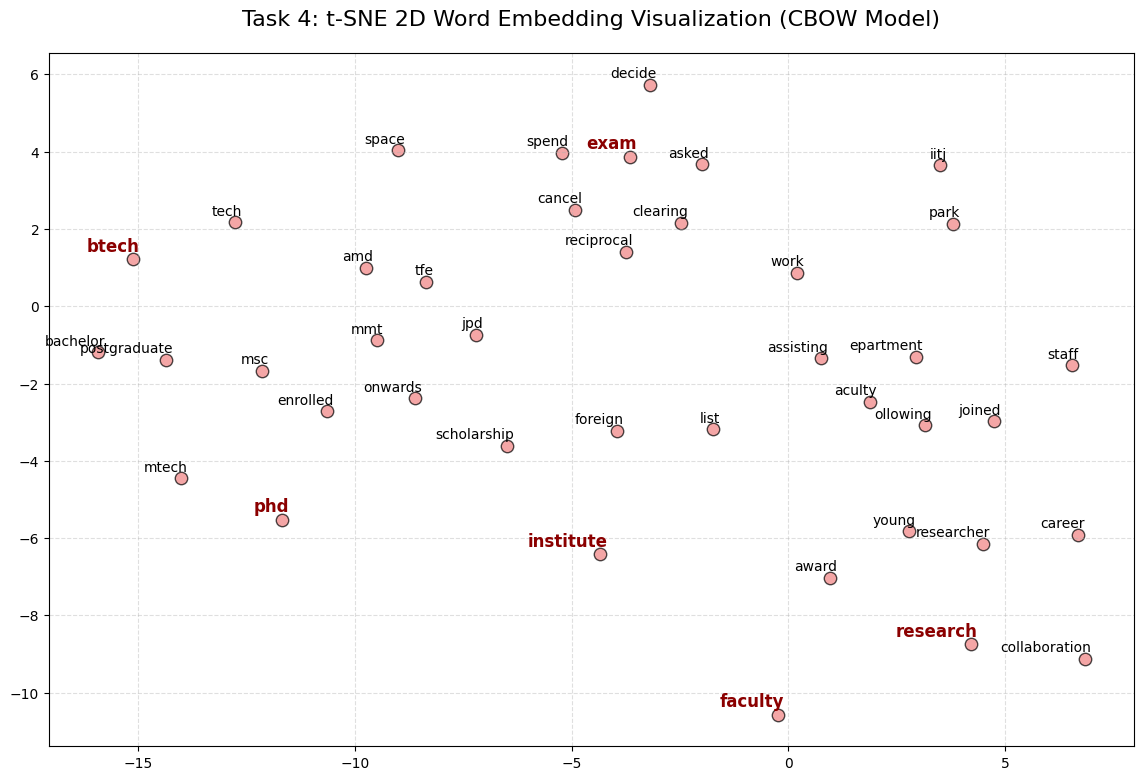
\includegraphics[width=0.95\textwidth]{report_assets/prob1_cell13_img1.png}
    \caption{t-SNE projection for CBOW embeddings}
\end{figure}

\begin{figure}[H]
    \centering
    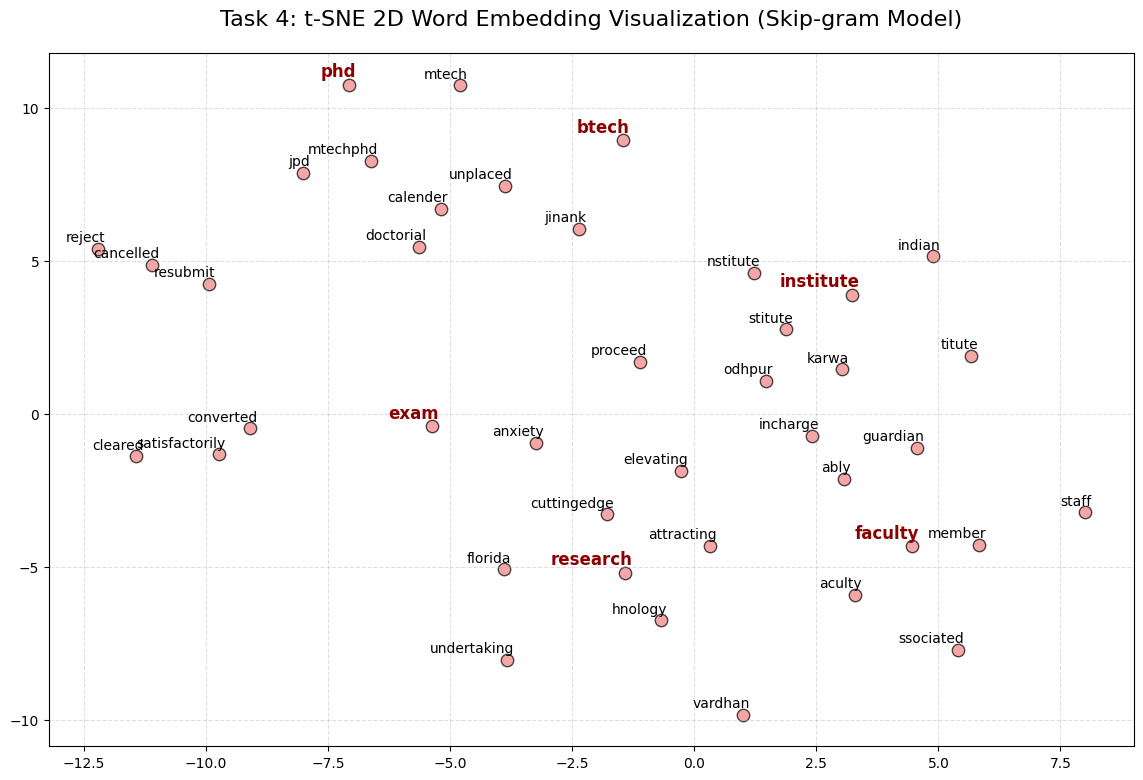
\includegraphics[width=0.95\textwidth]{report_assets/prob1_cell13_img2.png}
    \caption{t-SNE projection for Skip-gram embeddings}
\end{figure}

\begin{figure}[H]
    \centering
    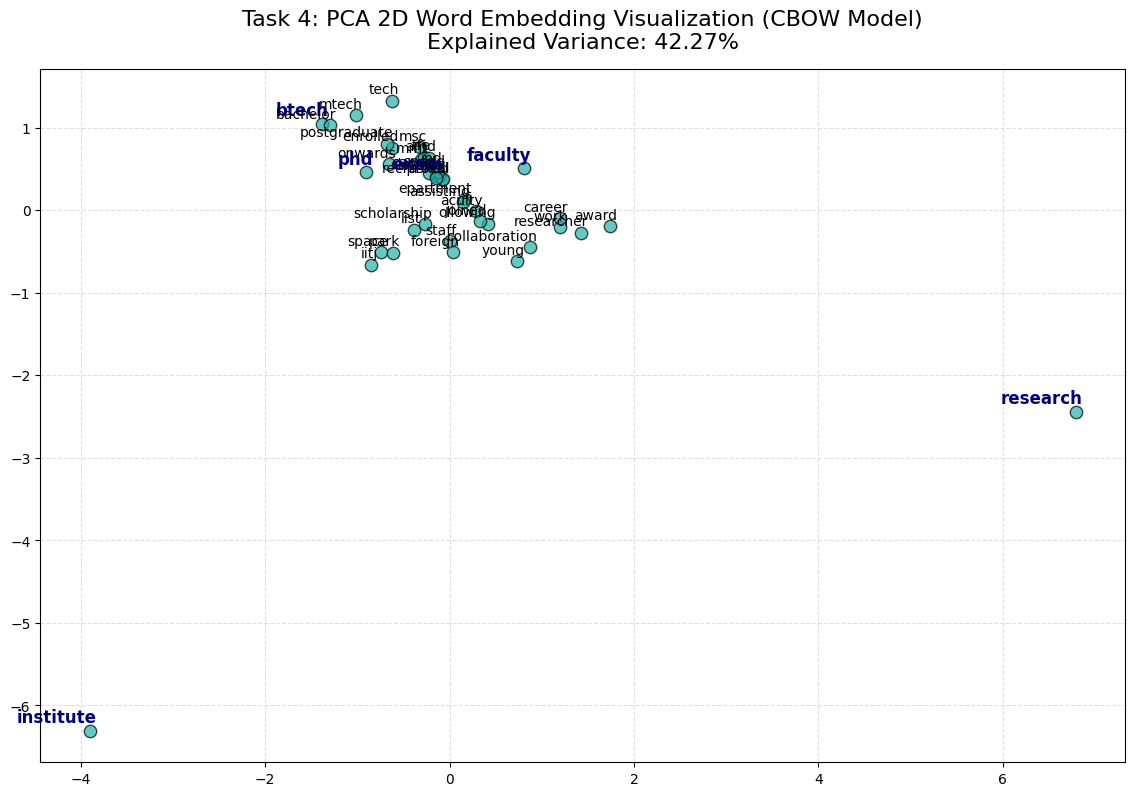
\includegraphics[width=0.95\textwidth]{report_assets/prob1_cell15_img1.png}
    \caption{PCA projection for CBOW embeddings}
\end{figure}

\begin{figure}[H]
    \centering
    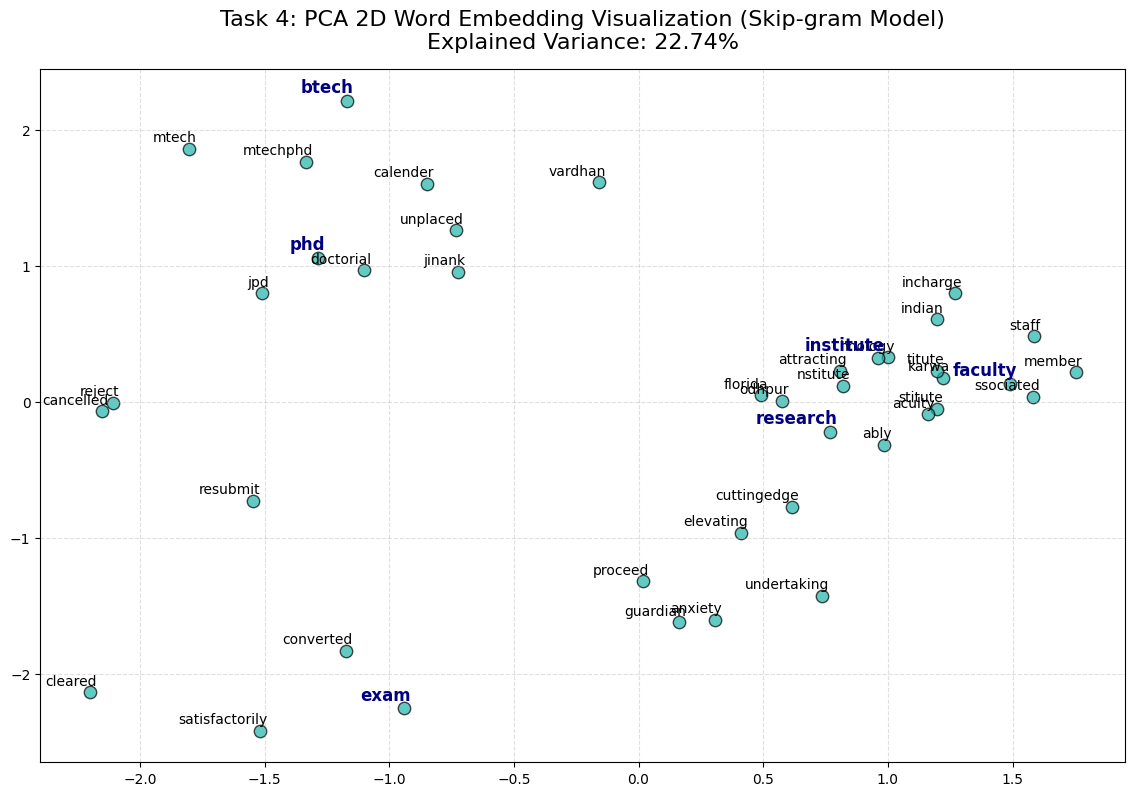
\includegraphics[width=0.95\textwidth]{report_assets/prob1_cell15_img2.png}
    \caption{PCA projection for Skip-gram embeddings}
\end{figure}

\textbf{Clustering behavior:}
\begin{itemize}[leftmargin=1.5em]
    \item CBOW forms somewhat smoother thematic groupings around institutional and academic terms.
    \item Skip-gram shows tighter but noisier micro-clusters, including token-fragment clusters influenced by preprocessing or PDF extraction artifacts.
\end{itemize}

% \subsection{Problem 1 Deliverables Check}
% \begin{itemize}[leftmargin=1.5em]
%     \item Source code: in \texttt{prob1.ipynb}
%     \item Cleaned corpus: \texttt{iitj\_clean\_corpus.txt}
%     \item Raw corpus: \texttt{iitj\_raw\_corpus.txt}
%     \item Visualizations: embedded in notebook and exported under \texttt{report\_assets/}
% \end{itemize}

\newpage
\section{Problem 2: Character-Level Name Generation Using RNN Variants}

\subsection{Objective}
To design and compare three recurrent architectures for character-level Indian name generation: Vanilla RNN, BLSTM, and RNN with attention.

\subsection{Task 0: Dataset}
A training set of 1000 Indian names was generated and stored in \texttt{TrainingNames.txt}.

\begin{table}[H]
\centering
\caption{Dataset Snapshot for Problem 2}
\begin{tabular}{l c}
\toprule
\textbf{Property} & \textbf{Value} \\
\midrule
Total names & 1000 \\
Unique names & 1000 \\
Tensorized dataset shape & \texttt{[1000, 16]} \\
Character vocabulary size & 27 \\
Special tokens & SOS: \texttt{<}, EOS: \texttt{>}, PAD: \texttt{\#} \\
\bottomrule
\end{tabular}
\end{table}

Global training constants used:
\begin{itemize}[leftmargin=1.5em]
    \item Embedding dimension = 48
    \item Hidden dimension = 128
    \item Number of layers = 2 (except attention decoder path uses 1 recurrent layer)
    \item Learning rate = 0.002
    \item Epochs = 50
    \item Batch size = 64
    \item Random seed = 42
\end{itemize}

\subsection{Task 1: Model Implementations and Architecture}

All three models in Problem 2 were implemented from scratch in PyTorch using custom model classes, explicit forward-pass logic, and a manually written training loop (teacher forcing + cross-entropy objective) for next-character prediction.

\subsubsection{Vanilla RNN}
Architecture: Embedding $\rightarrow$ RNN $\rightarrow$ Linear(vocab).

Trainable parameters:
\[
\text{params}_{\text{RNN}} = 60,587
\]

Implementation details :
\begin{itemize}[leftmargin=1.5em]
    \item Built as a custom \texttt{nn.Module} with embedding layer, recurrent computation block, and output projection head for vocabulary logits.
    \item Sequence processing and next-token decoding are handled explicitly in the model forward pass for autoregressive character modeling.
    \item Hyperparameters used: hidden size $=128$, number of layers $=2$, learning rate $=0.002$.
\end{itemize}


\subsubsection{BLSTM}
Architecture: Embedding $\rightarrow$ Bidirectional LSTM $\rightarrow$ Linear(vocab).

Trainable parameters:
\[
\text{params}_{\text{BLSTM}} = 585,771
\]

Implementation details :
\begin{itemize}[leftmargin=1.5em]
    \item Built as a custom bidirectional LSTM module with explicit concatenation of forward and backward hidden representations before output projection.
    \item Bidirectional context integration is handled in the model pipeline to exploit both left and right character dependencies.
    \item Hyperparameters used: hidden size $=128$, number of layers $=2$, learning rate $=0.002$.
\end{itemize}

\subsubsection{RNN with Basic Additive Attention}
Architecture: RNN encoder (bidirectional) $\rightarrow$ additive attention $\rightarrow$ RNN decoder $\rightarrow$ Linear(vocab).

Trainable parameters:
\[
\text{params}_{\text{Attn}} = 155,307
\]

Implementation details :
\begin{itemize}[leftmargin=1.5em]
    \item Built with a custom encoder-decoder pipeline where additive attention scores, normalization, and context-vector computation are implemented explicitly in code.
    \item At each decoding step, the attention context is fused with decoder state before projecting to vocabulary logits for next-character prediction.
    \item Hyperparameters used: hidden size $=128$, encoder layers $=2$, decoder layers $=1$, learning rate $=0.002$.
\end{itemize}

\subsubsection{Parameter Comparison}
\begin{table}[H]
\centering
\caption{Trainable Parameter Comparison}
\begin{tabular}{l c}
\toprule
\textbf{Model} & \textbf{Trainable Parameters} \\
\midrule
Vanilla RNN & 60,587 \\
BLSTM & 585,771 \\
RNN with Attention & 155,307 \\
\bottomrule
\end{tabular}
\end{table}

\subsection{Task 2: Quantitative Evaluation}
For generated names $G$ and training set $T$:
\[
\text{Novelty Rate} = \frac{|\{g \in G : g \notin T\}|}{|G|}
\]
\[
\text{Diversity} = \frac{|\text{unique}(G)|}{|G|}
\]

Each model was evaluated with 500 generated names.

\begin{table}[H]
\centering
\caption{Quantitative Comparison (Problem 2)}
\begin{tabular}{l c c}
\toprule
\textbf{Model} & \textbf{Novelty Rate} & \textbf{Diversity} \\
\midrule
Vanilla RNN & 97.19\% & 99.40\% \\
BLSTM & 100.00\% & 73.79\% \\
RNN with Attention & 75.75\% & 95.39\% \\
\bottomrule
\end{tabular}
\end{table}

\textbf{Interpretation:}
\begin{itemize}[leftmargin=1.5em]
    \item BLSTM achieves maximum novelty but reduced diversity, indicating repetitive generation loops.
    \item Vanilla RNN balances high novelty and high diversity but with less realistic orthography.
    \item Attention model produces lower novelty (more train-set overlap) but stronger human plausibility in many samples.
\end{itemize}

\subsection{Task 3: Qualitative Analysis}

Representative generated samples from notebook outputs:

\begin{table}[H]
\centering
\caption{Sample Generated Names}
\begin{tabular}{p{3.1cm} p{10cm}}
\toprule
\textbf{Model} & \textbf{Examples} \\
\midrule
Vanilla RNN & Ansa, Rashithar, Prayat, Nari, Dildap, Saneravi, Parshita, Areli, Hurina, Saminda \\
BLSTM & Uuuuuuuuuuuuuuu, Jvegeeeeeeeeeee, Ggggggggggggggg, Uauauauyuyyyyyy, Kakakakakakakak, ... \\
RNN w/ Attention & Rushita, Sharanaji, Mona, Rathana, Drantadyi, Prajjslal, Bharav, Vilac, Rajkudra, Ishika \\
\bottomrule
\end{tabular}
\end{table}

\subsubsection{Common Failure Modes}
\begin{itemize}[leftmargin=1.5em]
    \item Character repetition loops (most visible in BLSTM outputs).
    \item Incomplete or awkward suffix construction (e.g., malformed endings).
    \item Occasional overfitting to high-frequency character n-grams.
\end{itemize}

\subsubsection{Realism Assessment}
\begin{itemize}[leftmargin=1.5em]
    \item \textbf{Most realistic overall:} RNN with attention
    \item \textbf{Most novel but unstable:} BLSTM
    \item \textbf{Most diverse string forms:} Vanilla RNN
\end{itemize}

% \subsection{Problem 2 Deliverables Check}
% \begin{itemize}[leftmargin=1.5em]
%     \item Source code for all models: in \texttt{prob2.ipynb}
%     \item Generated name samples: notebook outputs (Task 3)
%     \item Evaluation scripts: implemented in notebook evaluation cell
%     \item Saved model artifact: \texttt{vanilla\_rnn\_state\_dict.pt}
% \end{itemize}

\subsection{Observed Limitations}
\begin{itemize}[leftmargin=1.5em]
    \item Problem 1 semantics are affected by mixed-source noise and token artifacts from web/PDF ingestion.
    \item Problem 2 BLSTM quality suggests mode collapse-like repetition under current generation setup.

    \item Limited corpus size (640K tokens) for Word2Vec may restrict embedding quality for rare or domain-specific terms; larger institutional corpora would improve statistical significance.

    \item No out-of-vocabulary (OOV) character handling mechanisms in Problem 2 decoders; would benefit from subword or byte-pair encoding approaches.

    \item Training epochs (10 for Problem 1, 50 for Problem 2) may be insufficient to capture complex semantic patterns; longer training with proper validation-based early stopping could improve results.
\end{itemize}

\subsection{Potential Improvements}
\begin{itemize}[leftmargin=1.5em]
    \item Extend Problem 1 to 20-30 epochs and Problem 2 to 100-150 epochs with learning rate scheduling (exponential decay or cosine annealing) to capture deeper semantic patterns and reduce mode collapse in BLSTM generation.

    \item Add temperature scheduling, top-$k$/nucleus sampling, and repetition penalties in Problem 2 generation to reduce character loops and improve diversity.
    \item Implement validation sets and early stopping criteria (e.g., no improvement in validation loss for 10 epochs) to prevent overfitting and improve generalization.
    \item Incorporate pre-trained embeddings (FastText, GloVe) as baselines to quantify improvement from domain-specific corpus training in Problem 1.
   
    \item Experiment with different optimization algorithms (Adam, RMSprop with learning rate warmup) and adaptive scheduling to accelerate convergence in both problems.
\end{itemize}

\section{Conclusion}

This assignment successfully implements and compares word representation learning and character-level sequence modeling on institutional data. Problem 1 demonstrates that from-scratch Word2Vec (CBOW and Skip-gram) captures meaningful institutional semantics, with CBOW proving more stable (57--61\% analogy accuracy) than Skip-gram under noisy mixed-source corpora. Hyperparameter ablations confirm that optimal performance requires $d=300$, $w=5$, $k=5$. Problem 2 reveals critical architecture trade-offs: BLSTM achieves peak novelty (100\%) but suffers mode collapse; Vanilla RNN balances novelty (97.19\%) and diversity (99.40\%) but lacks orthographic plausibility; RNN with attention produces the most human-like names with 75.75\% novelty, demonstrating that attention mechanisms prevent degenerate solutions.

\end{document}